\documentclass[11pt,a4paper]{article}
\usepackage[margin=24mm]{geometry}
\usepackage{fontspec}
\setmainfont[Path=fonts/]{ipaexg.ttf}
\setmonofont[Path=fonts/]{DejaVuSansMono.ttf}
\newfontfamily\jfont[Path=fonts/]{ipaexg.ttf}
\XeTeXlinebreaklocale "ja"
\XeTeXlinebreakskip=0pt plus 1pt
\usepackage{amsmath,amssymb,amsthm,mathtools}
\usepackage{graphicx,booktabs,hyperref}
\usepackage{fvextra}
\hypersetup{hidelinks}
\newtheorem{theorem}{定理}
\newcommand{\C}{\mathbb{C}}
\newcommand{\ket}[1]{\lvert #1\rangle}
\title{極端特異値推定におけるべき乗法とコサイン・フィルタ\\
QSVT提案の仮定を明示した技術的再評価}
\author{[著者名・所属を記入]}
\date{内部確認用技術報告草稿\\2026年10月26日}
\begin{document}
\maketitle
{\jfont
\begin{abstract}
未公開の量子最大・最小特異値推定案、とくにコサインを用いる「三角反復法」を再評価する。長方形行列 $A$ に対し、正規化右Gram作用素 $G=(A/\alpha)^\dagger(A/\alpha)$ 上に方法を定式化する。ここで $\alpha\geq\|A\|$ は利用可能な正規化上界である。$\cos(\beta G)$ の有界な偶多項式近似は、固有値多項式変換の候補となるが、具体的な実装にはQSP completion、実部の抽出、および正規化規約が必要である。本報告ではそれらの位相列・回路を構成しない。最小固有値の固有空間に入力確率 $a>0$ があり、最大の非目標応答が目標応答の $r<1$ 倍以下なら、$t$ 回反復後の条件付き漏れが $(1-a)r^{2t}/a$ 以下となる有限スペクトルの境界を示す。また、Bernoulli型ブロックエンコーディング読出しからフィルタ後のGram期待値を推定し、その加法誤差を特異値誤差へ換算する。境界は目標重なり、スペクトル分離、受理確率、正規化、読出し精度に依存し、回路全体やエンドツーエンドの計算量定理ではない。小行列の行列レベル計算は、重なりゼロ、狭いギャップ、右核に対する収束と失敗を再現する。原案の $\cos(\beta(\sigma/\alpha)^2)$ 応答と、別方式である拡張行列に基づく $\cos(\beta\sigma/\alpha)$ 応答も比較する。新規性や量子高速化は主張しない。
\end{abstract}

\section{はじめに}
最大・最小特異値は数値線形代数に現れ、基底状態エネルギー推定に関係するスペクトル問題にもつながる。先行する未公開原稿『量子最大・最小特異値推定アルゴリズム』（原稿コピーに著者・公開先等の書誌情報なし。以下QMSVE）は、最大特異値に対する量子べき乗法、最小値に対する逆反復法との比較、逆行列を明示的に適用しないコサイン型「三角反復法」を提案している\cite{QMSVE}。本報告は右空間の作用素上でその案を明確化し、収束条件を記録し、有限次元の小例を確認する。

中心となる修正は変換対象である。一般の長方形行列に $\cos(A)$ を直接適用しても特異値変換とはならない。そこで $B=A/\alpha$、$G=B^\dagger B$ とし、右特異ベクトル空間で考える。QMSVEのコサイン則は $C=\cos(\beta G)$ となり、その固有値は $\cos(\beta\sigma_i^2/\alpha^2)$ である。$0<\beta<\pi/2$ なら正規化スペクトル上で正かつ単調減少する。エルミート拡張行列から得られる $\cos(\beta\sigma_i/\alpha)$ は別の応答であり、原案の方式と区別する。

本報告の成果は、条件付きフィルタ収束、測定値から特異値への誤差換算、および再現可能な行列レベル監査を明示することにある。原案の新規性、全資源評価の正しさ、既存法に対する優位性は示さない。特にギャップと初期重なりが必要であり、フィルタ後の状態を受理するために多数の再試行が必要となる場合がある。

\section{関連研究と本報告の範囲}
量子特異値変換（QSVT）はブロックエンコードされた行列の特異値へ有界多項式変換を適用し、エルミートの場合には固有値多項式変換を実現する\cite{Gilyen}。ここではコサイン多項式の実装候補として位置づけ、位相角列は合成しない。量子べき乗法および量子逆反復法には既存の研究がある\cite{SekiYunoki,Kyriienko,Nghiem}。入力・実装モデルはそれぞれ異なるが、べき乗法やQSVTによるべき乗自体の新規性は主張しない。

確認したQMSVE原稿は著者・掲載先の記載がない未公開資料であり、「三角反復法」に仮題を付している。本報告では再評価対象となるアイデアの原資料として扱い、検証済み定理や既発表成果とは見なさない。著者の別のQCG研究は関連する既存資産としてのみ引用し、本手法と混同しない\cite{QCG2023,QCG2024}。

\section{モデルとアルゴリズム}
$A\in\C^{m\times n}$、$m\geq n$ とし、既知の $\alpha\geq\|A\|_2>0$ を選ぶ。$B=A/\alpha$、$G=B^\dagger B$ と置く。$G$ の固有値を昇順に
\[
 0\leq\lambda_0\leq\lambda_1\leq\cdots\leq\lambda_{n-1}\leq1
\]
と並べると、$\lambda_i=\sigma_i(A)^2/\alpha^2$ である。ここでは右空間全体における最小特異値を対象とし、零特異値も含める。最小「非零」特異値には、核直交部分空間へのアクセス等、追加の仮定が必要となる。横長行列 ($m<n$) の右Gram作用素には必ず核が含まれ、同じ区別が必要である。

右特異ベクトル基底に展開した正規化入力を $\ket{\psi}=\sum_i c_i\ket{v_i}$ とし、$p_i=|c_i|^2$ とする。$0<\beta<\pi/2$ に対する理想コサインGramフィルタを
\[
 C=\cos(\beta G),\qquad q_i=\cos(\beta\lambda_i)\in(0,1]
\]
と定める。$t$ 回反復後の非正規化状態は $C^t\ket{\psi}$、理想受理確率は
\[
 Z_t=\|C^t\ket{\psi}\|^2=\sum_i p_iq_i^{2t}
\]
であり、受理後の規格化状態における各固有値の重みは $p_iq_i^{2t}/Z_t$ となる。これは正規化を明示した、右Gram作用素上のQMSVEコサイン則である。

\paragraph{多項式実装モデル}
整数 $m_0\geq0$ に対し
\[
 P_{m_0}(x)=\sum_{j=0}^{m_0}\frac{(-1)^j(\beta x)^{2j}}{(2j)!},\quad
 \delta_{m_0}=\frac{\beta^{2m_0+2}}{(2m_0+2)!},\quad
 \widetilde P_{m_0}(x)=\frac{P_{m_0}(x)}{1+\delta_{m_0}}
\]
とする。$P_{m_0}$ は奇数次係数が零である $2m_0+1$ 次までのMaclaurin多項式である。Taylorの定理と余弦の各導関数の絶対値が1以下であることから、$|x|\leq1$ において $|P_{m_0}(x)-\cos(\beta x)|\leq\delta_{m_0}$ を得る。したがって $|\widetilde P_{m_0}(x)|\leq1$、一様近似誤差は $2\delta_{m_0}/(1+\delta_{m_0})$ 以下である。$\widetilde P_{m_0}$ は偶数次 $2m_0$ の多項式であり、$G$ のブロックエンコーディングに対するQSVTフィルタ候補に必要な偶奇性と区間有界性を満たす\cite{Gilyen}。ただし、具体的な実装にはQSP completion、実部抽出、正規化規約が必要であり、これらの補助ビットや費用は本稿で確立しない。特異値変数 $\sigma/\alpha$ で表した $\widetilde P_{m_0}((\sigma/\alpha)^2)$ の次数は $4m_0$ である。

$B$ のブロックエンコーディングがあれば、積の構成により、補助ビットと反射を除き2回の $B$ 呼出しで $G=B^\dagger B$ のブロックエンコーディングを構成できる。$G$ の多項式変換1回の実際のオラクル費用を $d_G$、初期状態準備費用を $c_\psi$ と記すが、数値評価はしない。$t$ 回の変換をコヒーレントに行う深さは $t d_G$ に比例し、硬い深さ上限は次数だけでなく反復回数も制限する。正規化上界 $\alpha$ とその取得費用は入力であり、アルゴリズムが無料で出力する値ではない。

\section{有限スペクトル収束と読出し}
最小固有値の固有空間を $T=\{i:\lambda_i=\lambda_0\}$ とし、その初期質量を $a=\sum_{i\in T}p_i>0$ とする。$q_*=\cos(\beta\lambda_0)$ とおき、
\[
 q_i\leq r q_*\quad(i\notin T),\qquad 0\leq r<1
\]
を仮定する。コサインGram応答では、$\lambda_0$ より大きい固有値が存在する場合、$\lambda_+=\min\{\lambda_i:\lambda_i>\lambda_0\}$ とおけば $r=\cos(\beta\lambda_+)/\cos(\beta\lambda_0)<1$ となる。全空間が目標空間なら $F_t=1$ である。

\begin{theorem}[条件付きスペクトル漏れ]
任意の整数 $t\geq0$ について、$C^t\ket{\psi}/\sqrt{Z_t}$ における $T$ の確率質量を $F_t$ とすると
\[
 1-F_t\leq\frac{1-a}{a}r^{2t}
\]
が成り立つ。さらに $\mu_t=\langle C^t\psi|G|C^t\psi\rangle/Z_t$ とすると
\[
 0\leq\mu_t-\lambda_0
 \leq(1-\lambda_0)(1-F_t)
 \leq\frac{1-a}{a}r^{2t}
\]
である。
\end{theorem}

証明を付録に示す。Lean形式化は作業中であり、付録に正確な範囲とchecker状況を記す。有限重みと行列固有基底の対応、ブロックエンコーディング、および読出しの解釈は有限次元での導出であり、scalar theoremのLean形式化には含まれない。

\paragraph{有限次数多項式への十分条件}
有界多項式であることだけでは、目標固有値が最大応答になるとは限らない。厳密コサイン応答の非目標最大値を $q_{\rm out}=\max_{i\notin T}q_i$ とし、区間上一様誤差を $|\widetilde P(x)-\cos(\beta x)|\leq E$ とする。$E<(q_*-q_{\rm out})/2$ なら、$|\widetilde q_*|\geq q_*-E>0$、かつ $|\widetilde q_i|/|\widetilde q_*|\leq(q_{\rm out}+E)/(q_*-E)<1$ である。同じ有限重み境界がこの比で成り立つ。これは十分条件であり、次数最適性は評価していない。

\paragraph{最大特異値に対するべき乗法}
最大値側では応答を $q_i=\lambda_i$、目標を $T_{\max}=\{i:\lambda_i=\lambda_{\max}\}$ とする。初期質量 $a_{\max}>0$、$\lambda_{\max}>0$ とし、$\lambda_-=\max\{\lambda_i:\lambda_i<\lambda_{\max}\}$ がある場合、同じ有限重み不等式を $q_*=\lambda_{\max}$、$r=\lambda_-/\lambda_{\max}$ に適用できる。フィルタ後の平均には $0\leq\lambda_{\max}-\mu_t\leq(1-F_t)\leq((1-a_{\max})/a_{\max})r^{2t}$ が成り立つ。$G$のブロックエンコーディングのBernoulli読出しを同様に行えば、$\sigma_{\max}(A)$ の誤差は $\alpha\sqrt{((1-a_{\max})/a_{\max})r^{2t}+\zeta}$ 以下となる。$\lambda_{\max}<1$ なら受理確率は $\lambda_{\max}^{2t}$ 以下にもなり得る。最大値への条件付き集中にも成功コストがある。

ブロックエンコーディングされた $B$ の成功フラグを、受理状態 $\ket{\psi_t}$ に対して読み、フラグで再びpostselectしない場合、Bernoulli平均は $\langle\psi_t|B^\dagger B|\psi_t\rangle=\mu_t$ である。受理後状態を $M$ 個独立に準備し、$M\geq\log(2/\delta)/(2\zeta^2)$ とすれば、Hoeffding不等式より確率 $1-\delta$ で $|\widehat\mu_t-\mu_t|\leq\zeta$ となる。$\widehat\mu_t$ を $[0,1]$ にclipし、$\widehat\sigma=\alpha\sqrt{\widehat\mu_t}$ とすれば
\[
 |\widehat\sigma-\sigma_0(A)|
 \leq \alpha\sqrt{\frac{1-a}{a}r^{2t}+\zeta}
\]
である。これは理想Bernoulli読出しでの加法誤差であり、ノイズ、状態準備誤差、未知の $\alpha$ は含まない。

\paragraph{受理確率と費用}
理想コサイン応答では $a q_*^{2t}\leq Z_t\leq q_*^{2t}$ であり、失敗試行ごとに初期状態から再開すれば、受理コピー1個あたりの試行期待値は $1/Z_t$ である。実装多項式応答 $\widetilde P$ の応答を $\widetilde q_i$ とすると、対応する理想スペクトルノルム確率は $\widetilde Z_t=\sum_i p_i|\widetilde q_i|^{2t}$ となる。さらにQSP completion等が応答にスカラー係数 $c\in(0,1]$ を与える場合、実際の枝の成功確率は $c^{2t}\widetilde Z_t$ である。この係数と位相列は本稿では確定しない。したがって費用proxyは、該当する実際の成功確率を $P_t^{\rm succ}$ として
\[
 M\left(\frac{c_\psi+t d_G}{P_t^{\rm succ}}+d_B\right)
\]
と書く。$d_B$ は1回のBernoulli読出しに使う $B$ ブロックエンコーディング費用である。振幅増幅、コヒーレントな再利用、コンパイル済みゲート費用は未計上。理想コサインの場合、$\lambda_0>0$ なら $q_*<1$ で受理確率は反復回数とともに指数減衰し得る。条件付き漏れが小さいことだけでは総費用が小さいとは言えない。

\section{数値結果}
7個の小行列について右Gram作用素を古典的に固有値分解し、固定したスペクトル重みを用いる決定論的な行列レベル計算を行った。入力状態は計算した右固有ベクトル基底で定義し、固有値応答で重みを更新する。これは固有状態を使った制御スペクトル監査であり、未知の特異ベクトルを準備する性能評価ではない。量子状態ベクトルや量子回路はシミュレートしていない。図は $\beta=1.2$ における厳密な $\cos(\beta G)$ 応答を示す。別途、seed 20261026、受理後2,000 Bernoulli標本の読出しを行った。コードと完全なJSON結果は \texttt{experiments/qmsve\_matrix\_level.py} と \texttt{results/qmsve\_matrix\_level.json} にある。

\begin{figure}[t]
\centering
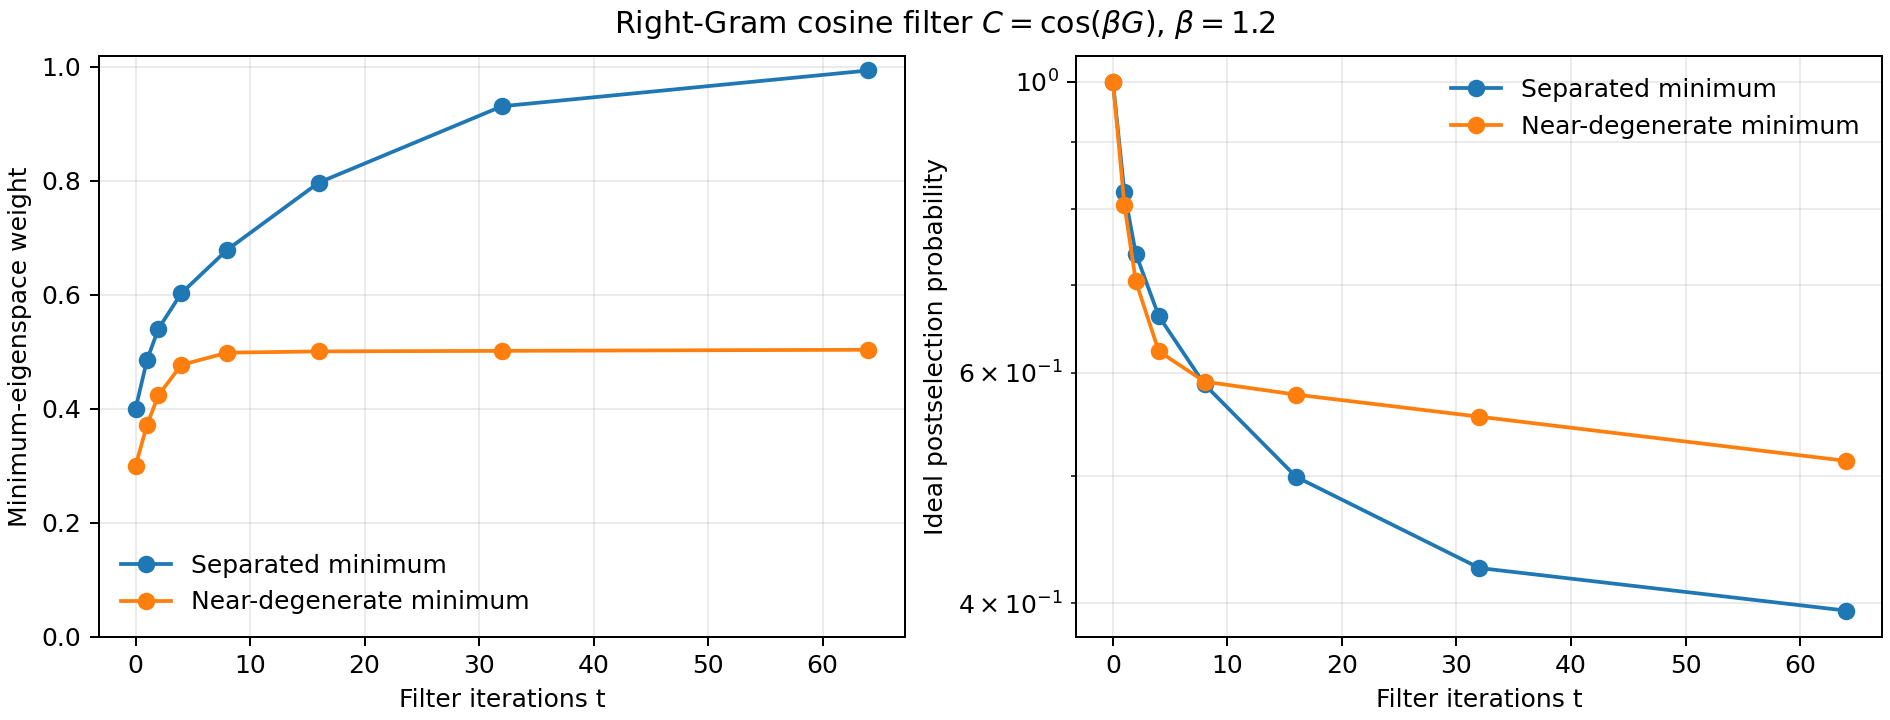
\includegraphics[width=\linewidth]{../../figures/qmsve_matrix_level.png}
\caption{行列レベル計算による条件付き目標質量と理想フィルタ受理確率。特異値ギャップのある例では最小固有空間へ集中するが、近縮退例は表示した反復数では十分集中しない。}
\label{fig:filter-ja}
\end{figure}

\begin{center}
\scriptsize
\begin{tabular}{lrrrrr}
\toprule
例 & $\sigma_{\min}$ & $a_{\min}$ & $G^8$ 推定値 & $\cos(\beta G)^8$ 推定値 / 質量 & $\cos(\beta\sqrt G)^8$ 推定値 / 質量\\
\midrule
正方・分離ギャップ & 0.12 & 0.40 & 0.8600 & 0.2896 / 0.6791 & 0.1643 / 0.9417\\
近縮退 & 0.20 & 0.30 & 0.8000 & 0.2076 / 0.4987 & 0.2027 / 0.5059\\
縮退最小値 & 0.20 & 0.40 & 0.7000 & 0.2713 / 0.9254 & 0.2041 / 0.9963\\
目標重なりゼロ & 0.12 & 0 & 0.8600 & 0.4809 / 0 & 0.4803 / 0\\
横長・行フルランク & 0 & 0.16 & 0.8000 & 0.2744 / 0.5666 & 0.1442 / 0.8715\\
階数落ち正方 & 0 & 0.30 & 0.8000 & 0.2654 / 0.5714 & 0.1435 / 0.8719\\
回転した縦長行フルランク & 0.15 & 0.35 & 0.6500 & 0.3065 / 0.8214 & 0.1630 / 0.9898\\
\bottomrule
\end{tabular}
\end{center}
$G^8$ 列は最大特異値推定、コサイン列は最小特異値推定値と条件付き最小固有空間質量である。正方ギャップ例で $G^8$ の理想受理確率は $0.00200$、コサインGram応答では $0.5876$ である。条件付き推定値と受理サンプルの費用を混同してはならない。

正方ギャップ例の $t=8$ におけるTaylor多項式応答は次の通りである。
\begin{center}
\small
\begin{tabular}{rrrrrr}
\toprule
$G$上次数 & $\sigma/\alpha$上次数 & 一様誤差上界 & $\widehat\sigma$ & 目標質量 & 理想受理確率\\
\midrule
2 & 4 & $1.591\times10^{-1}$ & 0.2891 & 0.6801 & 0.1558\\
4 & 8 & $8.260\times10^{-3}$ & 0.2896 & 0.6791 & 0.5499\\
6 & 12 & $2.133\times10^{-4}$ & 0.2896 & 0.6791 & 0.5866\\
12 & 24 & $2.946\times10^{-10}$ & 0.2896 & 0.6791 & 0.5876\\
\bottomrule
\end{tabular}
\end{center}
これらは解析的一様有界性余裕を持つ多項式応答の計算であり、QSVT位相角列の合成結果ではない。表の受理確率もコンパイル回路の測定値ではなく、理想スペクトル応答の計算値である。

$t=64$ では、分離ギャップ例 $(0.12,0.48,0.86)$ の最小固有空間質量は $0.994$、理想受理確率は $0.395$ である。近縮退例 $(0.20,0.205,0.80)$ は質量 $0.504$、受理確率 $0.514$ にとどまる。目標初期質量が $0.40$ の縮退最小値は $0.999999$ より大きい質量に達するが、選ばれるのは固有空間であり特定のベクトルではない。最小固有空間への初期重なりがゼロの場合、フィルタはその成分を生成できない。実験例では推定値は $0.48$ にとどまり、理想受理確率は $0.00282$ まで減少する。

横長の行フルランク行列では右Gram作用素に零固有値があり、方法は最小非零特異値ではなく右核を対象にする。階数落ち正方行列でも最小値は零である。宣言した $\alpha=1$ より行列ノルムが大きい入力は正規化検査で拒否される。

正方ギャップ例の $t=8$ における厳密なフィルタ後Gram平均は $0.08385$ であった。2,000標本のBernoulli平均は $0.0780$ で、失敗確率 $0.05$ のHoeffding半径 $0.03037$ 内にある。2,000個の受理標本を得るまでの理想期待試行回数は約3,404回である。これは条件付きBernoulliモデルの確認であり、量子回路の実行ではない。

別方式の $\cos(\beta\sigma/\alpha)$ は分離ギャップ例では $t=16$ に目標質量 $0.996$（原案の $\cos(\beta(\sigma/\alpha)^2)$ は $0.797$）へ達する一方、受理確率はそれぞれ $0.288$ と $0.500$ である。近縮退例では両応答とも $t=16$ で質量は約 $0.5$ にとどまる。多項式次数、エンコーディング、コンパイル費用を一致させた比較ではない。

\section{考察と限界}
有限スペクトルの議論は、目標固有空間でフィルタ応答が厳密に最大なら他の重みが幾何的に抑圧されることを示す。同じ計算は応答比の仮定を満たす他の対角フィルタにも当てはまるため、この漏れ不等式自体を新しい量子アルゴリズムと解釈すべきではない。実用上の問いは、選んだ応答を適切な多項式次数で実装できるか、深さ・問い合わせ予算内に十分な受理標本を得られるかである。本報告はこのエンドツーエンド最適化を解決していない。

目標固有空間への初期質量は正でなければならず、有用な保証にはその下界が必要である。また $r<1$ の応答比が必要であり、コサインGramフィルタでは最小値より上のスペクトルギャップから従う。反復postselectionは $1/Z_t$ の期待オーバーヘッドを生じ、目標固有値が正なら成功確率は反復回数とともに指数的に小さくなる場合がある。正規化 $\alpha$ の取得費用は含まない。Taylor応答は指定区間で有界だが、位相合成、有限精度誤差の反復伝播、ノイズは評価していない。

数値例は縮退、狭いギャップ、重なりゼロ、右核を示すための小例であり、化学系、大規模疎行列、実機性能を示さない。量子高速化、問い合わせ計算量の改善、新規性は主張しない。実資源比較には共通入力モデル、状態準備、正規化、ブロックエンコーディング、フィルタ次数、成功増幅または再試行、読出し標本数、有限精度誤差を含める必要がある。

\section{結論}
正規化右Gram作用素上でQMSVEコサイン反復法を仮定明示的に定式化し、有限スペクトルでの条件付き収束とBernoulli読出し保証を示した。再現可能な小行列計算はギャップ、目標重なり、縮退、重なりゼロ、右核の役割を示した。条件付き収束だけでは効率的なアルゴリズムを確立できず、成功確率と実装費用も計上しなければならない。本検討ではエンドツーエンドの資源優位を確立していない。

\appendix
\section{有限スペクトル境界の証明}
目標部分空間の非正規化質量を $Q_T=aq_*^{2t}$、それ以外を $Q_\perp=\sum_{i\notin T}p_iq_i^{2t}$ とする。応答比の仮定から $Q_\perp\leq(1-a)r^{2t}q_*^{2t}$ であり、$Z_t=Q_T+Q_\perp\geq aq_*^{2t}$ である。したがって
\[
 1-F_t=\frac{Q_\perp}{Q_T+Q_\perp}
 \leq\frac{Q_\perp}{Q_T}
 \leq\frac{1-a}{a}r^{2t}.
\]
目標外の固有値は全て $[\lambda_0,1]$ にあるため
\[
 \mu_t-\lambda_0
 =\sum_{i\notin T}\frac{p_iq_i^{2t}}{Z_t}(\lambda_i-\lambda_0)
 \leq(1-F_t)(1-\lambda_0)
 \leq\frac{1-a}{a}r^{2t}.
\]

\section{Taylor余弦近似}
$x\in[-1,1]$ における余弦Taylor多項式の誤差は
\[
 |P_{m_0}(x)-\cos(\beta x)|\leq
 \delta_{m_0}=\frac{\beta^{2m_0+2}}{(2m_0+2)!}
\]
である。よって $|P_{m_0}(x)|\leq1+\delta_{m_0}$ であり、$\widetilde P_{m_0}$ は全区間で絶対値1以下となる。近似誤差は $2\delta_{m_0}/(1+\delta_{m_0})$ 以下である。この一様境界は数値グリッドだけからの推測ではない。

\section{Lean形式化の対応と範囲}
Lean付録では、有限重みの漏れ不等式と事後Gram期待値の逸脱境界を形式化する。目標総質量 $a>0$、目標応答 $q_*>0$、目標外応答が $r q_*$ 以下のとき、漏れは $((1-a)/a)r^{2t}$ 以下となる。完全なLeanソースを付録に掲載し、Lean 4.35.0、Mathlib v4.35.0で確認した。\texttt{lake build QMSVE} と \texttt{lake env lean Audit.lean} はともにexit code 0である。実行記録はソース一式に含む。行列対角化とQSVTから有限確率重みへの同定は手証明による。量子回路、ブロックエンコーディング、SVD、Hoeffding集中全体をLean検証済みとは扱わない。

\section{原資料の書誌情報}
利用したQMSVE原稿の題名は『量子最大・最小特異値推定アルゴリズム』である。確認したコピーには著者、所属、公開先の記載がなく、「三角反復法」は仮題とされる。本文の著者情報は未確定とし、人物・所属は推定しない。
\section{Lean証明ソース}
以下に本文の有限重み不等式と事後期待値境界を検証した完全なLeanソースを掲載する。プロジェクトの固定版と再現可能なchecker commandは同梱READMEに記す。
\VerbatimInput[fontsize=\tiny,breaklines=true]{../../lean/QMSVE.lean}
\renewcommand{\refname}{参考文献}
\begin{thebibliography}{9}
\bibitem{QMSVE} \emph{Quantum maximum/minimum singular-value estimation algorithms}. Unpublished manuscript supplied as \texttt{2023\_0311\_QMSVE.pdf}; author and publication metadata unstated in the copy examined.
\bibitem{Gilyen} A. Gily\'en, Y. Su, G. H. Low, and N. Wiebe, "Quantum singular value transformation and beyond: exponential improvements for quantum matrix arithmetics," in \emph{Proceedings of the 51st Annual ACM SIGACT Symposium on Theory of Computing}, pp. 193--204 (2019), doi:10.1145/3313276.3316366; arXiv:1806.01838.
\bibitem{SekiYunoki} K. Seki and S. Yunoki, "Quantum Power Method by a Superposition of Time-Evolved States," \emph{PRX Quantum} \textbf{2}, 010333 (2021), doi:10.1103/PRXQuantum.2.010333; arXiv:2008.03661.
\bibitem{Kyriienko} O. Kyriienko, "Quantum inverse iteration algorithm for programmable quantum simulators," \emph{npj Quantum Information} \textbf{6}, 7 (2020), doi:10.1038/s41534-019-0239-7; arXiv:1901.09988.
\bibitem{Nghiem} N. A. Nghiem, H. Sukeno, S. Zhang, and T.-C. Wei, "Improved Quantum Power Method and Numerical Integration Using Quantum Singular Value Transformation," \emph{Physical Review A} \textbf{111}, 012434 (2025), doi:10.1103/PhysRevA.111.012434; arXiv:2407.11744.
\bibitem{QCG2023} K. Toyoizumi, S. Yamamoto, and Y. Hoshino, "Hamiltonian simulation using quantum singular value transformation: complexity analysis and application to the linearized Vlasov-Poisson equation," arXiv:2304.08937, version 2 (2023).
\bibitem{QCG2024} K. Toyoizumi, K. Wada, S. Yamamoto, and Y. Hoshino, "Quantum conjugate gradient method using the positive-side quantum eigenvalue transformation," arXiv:2404.02713, version 2 (2024).
\end{thebibliography}
}
\end{document}
